\title{Estimating population average treatment effects from experiments with noncompliance
\vspace{15mm}}

\author{Kellie Ottoboni\thanks{Department of Statistics, University of California, Berkeley. email: \href{mailto:kellieotto@berkeley.edu}{\nolinkurl{kellieotto@berkeley.edu}}.} \hspace{10mm}
Jason Poulos\thanks{Travers Department of Political Science, University of California, Berkeley. email: \href{mailto:poulos@berkeley.edu}{\nolinkurl{poulos@berkeley.edu}}.} 
\vspace{15mm}} 

\date{\today}

%%%%%%%%%%%%%%%%%%%%%%%%%%%%%%%%%%%%%%%%%%%%%%%%%%
% Set document class
\documentclass[12pt]{article}

% Define packages
\usepackage{graphicx,amsfonts,psfrag,layout,subcaption,array,longtable,lscape,booktabs,dcolumn,natbib,amsmath,amssymb,amssymb,amsthm,setspace,epigraph,chronology,color, colortbl,caption,wasysym}
\usepackage[]{graphicx}\usepackage[]{color}
\usepackage[page]{appendix}
\usepackage{hyperref, url} 
\usepackage[section]{placeins}
\usepackage[linewidth=1pt]{mdframed}
\usepackage[margin=1in]{geometry} %1 inch margins

% Footnotes stick at the bottom
\usepackage[bottom]{footmisc}

% New footnote characters
\usepackage{footmisc}
\DefineFNsymbols{mySymbols}{{\ensuremath\dagger}{\ensuremath\ddagger}\S\P
   *{**}{\ensuremath{\dagger\dagger}}{\ensuremath{\ddagger\ddagger}}}
\setfnsymbol{mySymbols}

% New tabular environment
\usepackage{tabularx}
\newcolumntype{Y}{>{\raggedleft\arraybackslash}X}% raggedleft column X

% Define appendix 
\renewcommand*\appendixpagename{Appendix}
\renewcommand*\appendixtocname{Appendix}

% Position floats
\renewcommand{\textfraction}{0.05}
\renewcommand{\topfraction}{0.95}
\renewcommand{\bottomfraction}{0.95}
\renewcommand{\floatpagefraction}{0.35}
\setcounter{totalnumber}{5}

% Colors for highlighting tables
\definecolor{Gray}{gray}{0.9}

% Different font in captions
\newcommand{\captionfonts}{\scriptsize}

\makeatletter  % Allow the use of @ in command names
\long\def\@makecaption#1#2{%
  \vskip\abovecaptionskip
  \sbox\@tempboxa{{\captionfonts #1: #2}}%
  \ifdim \wd\@tempboxa >\hsize
    {\captionfonts #1: #2\par}
  \else
    \hbox to\hsize{\hfil\box\@tempboxa\hfil}%
  \fi
  \vskip\belowcaptionskip}
%\makeatother   % Cancel the effect of \makeatletter
 
% Set Spacing
\doublespacing

%Theorem
\newtheorem{theorem}{Theorem}

% Number assumptions
\newtheorem*{assumption*}{\assumptionnumber}
\providecommand{\assumptionnumber}{}
\makeatletter
\newenvironment{assumption}[2]
 {%
  \renewcommand{\assumptionnumber}{Assumption #1}%
  \begin{assumption*}%
  \protected@edef\@currentlabel{#1}%
 }
 {%
  \end{assumption*}
 }
\makeatother

% Macros
\newcommand{\Adv}{{\mathbf{Adv}}}       
\newcommand{\prp}{{\mathrm{prp}}}                  % How to define new commands 
\newcommand{\calK}{{\cal K}}
\newcommand{\outputs}{{\Rightarrow}}                
\newcommand{\getsr}{{\:\stackrel{{\scriptscriptstyle\hspace{0.2em}\$}}{\leftarrow}\:}}
\newcommand{\andthen}{{\::\;\;}}    %  \: \; for thinspace, medspace, thickspace
\newcommand{\Rand}[1]{{\mathrm{Rand}[{#1}]}}       % A command with one argument
\newcommand{\Perm}[1]{{\mathrm{Perm}[{#1}]}}       
\newcommand{\Randd}[2]{{\mathrm{Rand}[{#1},{#2}]}} % and with two arguments
\newcommand{\E}{\mathrm{E}}
\newcommand{\ind}{\mathbb{I}} % Indicator function
\newcommand{\pr}{\mathbb{P}} % Generic probability
\newcommand{\ex}{\mathbb{E}} % Generic expectation
\newcommand{\Var}{\mathrm{Var}}
\newcommand{\Cov}{\mathrm{Cov}}
\newcommand{\cov}{\mathrm{Cov}}
\DeclareMathOperator*{\plim}{plim}
\newcommand\independent{\protect\mathpalette{\protect\independenT}{\perp}}
\def\independenT#1#2{\mathrel{\rlap{$#1#2$}\mkern2mu{#1#2}}}
\newcommand{\possessivecite}[1]{\citeauthor{#1}'s [\citeyear{#1}]} 
\newcommand{\todo}[1]{{\color{red}{TO DO: \sc #1}}}

% Making a DAG
\usepackage{tkz-graph}  
\usetikzlibrary{shapes.geometric}
\tikzstyle{VertexStyle} = [shape            = ellipse,
                               minimum width    = 6ex,%
                               draw]
 \tikzstyle{EdgeStyle}   = [->,>=stealth']      



\begin{document}
\begin{singlespace} % single space for cover
\maketitle  
\thispagestyle{empty}
\begin{abstract}  
\noindent 
We extend the method of \citet{Hartman} to identify population average treatment effects from randomized controlled trials (RCTs) with noncompliance. We identify the complier--average causal effect for the target population with few additional assumptions. Simulation results show the compliance--adjusted estimator performs better than the unadjusted estimator when compliance is relatively low and can be predicted by observed covariates. We apply the proposed estimator to measure the effect of Medicaid coverage on health care use for a target population of adults who may benefit from expansions to the Medicaid program. We draw RCT data from the Oregon Health Insurance Experiment \citep{finkelstein2012}, in which only $30\%$ of those randomly selected to receive Medicaid benefits actually enrolled. The RCT sample differs in several dimensions from the target population of individuals who will be covered by other Medicaid expansions. We find substantial differences between sample and population estimates in terms of race, education, and health status subgroups. 

\end{abstract}	
\end{singlespace}
%Move introduction to second page
\pagebreak
\setcounter{page}{1} % Reset to Page 1

\vspace{20mm}

\section{Introduction}
Randomized control trials (RCTs) are the gold standard for estimating the causal effect of a treatment.  An RCT may give an unbiased estimate of the sample average treatment effect (SATE), but external validity is an issue when the individuals in the RCT are unrepresentative of the actual population of interest.  For example, the participants in an RCT in which individuals volunteer to sign up for health insurance may be in poorer health at baseline than the overall population.  External validity is particularly relevant to policymakers who want to know how the SATE would generalize to the broader population. Hartman et al. propose a method of reweighting the responses of individuals in an RCT according to the distribution of covariates in the target population in order to estimate the population average treatment effect on the treated (PATT).  Under a series of assumptions, the PATT is identified from the RCT outcomes \citep{Hartman}. 

A prevalent issue in RCTs is noncompliance.  One-way crossover from treatment to control occurs when individuals who are assigned to the treatment group refuse the treatment.  This dilutes the estimated effect of treatment assignment, and the resulting intention--to--treat (ITT) estimate is biased towards zero.  We extend the method of Hartman et al. to estimate the PATT from RCT data with noncompliance.  We make the same assumptions needed for the estimator proposed by \cite{Hartman}; these include the stable unit treatment value assumption and strong ignorability of sample assignment.  To deal with noncompliance, we follow the instrumental variables approach and make the no--defiers and exclusion restriction assumptions as in \cite{Angrist1996}. 

The proposed estimator of PATT involves the expectation of the response of compliers in the RCT sample, conditional on their covariates, where the expectation is taken over the distribution of population covariates.  We use a classification or regression model to estimate the response surface, the conditional expectation of responses in the RCT.  We then use the response model to estimate population members' outcomes given their covariates, giving an estimate of the PATT. 

The paper proceeds as follows: Section 2 presents the proposed estimator, necessary assumptions for its identifiability, and an estimation procedure; Section 3 investigates the estimator's performance in simulations; Section 4 uses the estimator to identify the effect of extending Medicaid coverage to the low--income adult population in the U.S; Section 5 discusses the results. 

\section{Estimator} \label{estimator}
We are interested in using the outcomes from an RCT to estimate the average treatment effect on the treated for a target population.  Treatment in the population is not assigned at random, but rather depends on other variables, confounding the effect of treatment on the outcome of interest. RCTs are needed to isolate the effect of treatment. However, strict exclusion criteria for RCTs often result in a sample whose distribution of covariates differs substantially from the target population.  Ideally, we would take the results of an RCT and reweight the sample such that the reweighted covariates match the those in the population. In practice, one rarely knows the true covariate distribution in the target population.  Instead, we consider data from a non-randomized, observational study in which participants are representative of the target population.  Our proposed estimator combines RCT and observational data to overcome these issues.

\subsection{Assumptions} 
Let $Y_{ist}$ be the potential outcome for individual $i$ in group $s$, where $s=0$ is the population and $s=1$ is the RCT, and $t$ be the treatment received.  Let $S_i$ denote the sample assignment, $T_i$ denote the treatment assigned, and $D_i$ denote treatment received. Let $W_i$ be individual $i$'s observable pretreatment covariates that are related to the sample selection mechanism for membership in the RCT, treatment assignment in the population, and complier status.  Let $C_i$ be an indicator for individual $i$'s compliance to treatment.  For a generic value, we drop the subscript $i$.  

Assuming that treatment is assigned at random in the RCT, we observe $D_i = T_i$ for individuals with $C_i = 1$.  In the population, we suppose that treatment is made available to individuals according to some rule based on their covariates; that is, treatment assignment is not completely random. Individuals with $T_i = 0$ do not receive treatment, while those with $T_i=1$ may decide whether or not to accept treatment.  We only observe $D_i$, not $T_i$, for individuals in the population.  Among the population controls, we can't distinguish non-compliers who should have received treatment (individuals with $T_i=1$ and $D_i = 0$) from those assigned to control (those with $T_i = 0$ and $D_i = 0$).  Compliance $C_i$ is only observable for individuals assigned to treatment in the RCT. 

Assumptions (\ref{consistency}) -- (\ref{sutva}) are made by \cite{Hartman} to identify PATT from an RCT. 

\begin{assumption}{1}{}\label{consistency}
Consistency under parallel studies: for all $i$ and for $t=0, 1$.
$$Y_{i0t} = Y_{i1t}$$
\end{assumption}

\noindent Assumption (\ref{consistency}) requires that each individual $i$ has the same response to treatments, whether $i$ is in the RCT or not. 

\begin{assumption}{2}{}\label{si_treat}
Strong ignorability of sample assignment for treated:
\begin{equation*}
(Y_{01}, Y_{11}) \independent S \mid (W, T=1,C = 1), 0 < \pr(S=1 \mid W, T=1,C = 1) <1.
\end{equation*}
\end{assumption}
\noindent Assumption (\ref{si_treat}) ensures the potential outcomes for treatment are independent of sample assignment for individuals with the same covariates $W$ and assignment to treatment. We make a similar assumption for controls: 

\begin{assumption}{3}{}\label{si_ctrl}
Strong ignorability of sample assignment for controls:
\begin{equation*}
(Y_{00}, Y_{10}) \independent S \mid (W, T=1,C = 1), 0 < \pr(S=1 \mid W, T=1,C = 1) <1. 
\end{equation*}\end{assumption}
 
\begin{assumption}{4}{}\label{sutva}
No interference between units: The potential outcomes $Y_{ist}$ for individual $i$, $s = 0,1$, $t=0,1$ do not depend on $T_j$, for all $j\neq i$. 
%\begin{equation*}
%Y_{ist}^{L_i} = Y_{ist}^{L_j},  \forall i \neq j

%\end{equation*}
%where $L_j$ is the treatment and sample assignment vector for unit $j$. 
\end{assumption} 

We include Assumption (\ref{compl}) among those made by \cite{Hartman} to ensure that compliance is independent of sample and treatment assignment for all individuals with covariates $W$. 
 
\begin{assumption}{5}{}\label{compl}
Conditional independence of compliance and assignment:
\begin{equation*}
C \independent T=1 \mid W, 0 < \pr(C = 1 \mid W) < 1. 
\end{equation*}
\end{assumption}

We additionally include Assumptions (\ref{monotonicity}) ---(\ref{ER}), which are made by \cite{Angrist1996} to ensure identifiability. The former assumption ensures that crossover is only possible from treatment to control.  The latter assumption ensures treatment assignment affects the response only through the treatment received.  In particular, the treatment effect may only be non-zero for compliers.

\begin{assumption}{6}{}\label{monotonicity}
No defiers: 
\begin{equation*}
T_i \geq D_i, \forall i. 
\end{equation*}
\end{assumption}

\begin{assumption}{7}{}\label{ER}
Exclusion restriction: For non-compliers
\begin{equation*}
Y_{11} = Y_{10}. 
\end{equation*}  
\end{assumption}

% fig:DAG

\subsection{Population Average Treatment Effect on the Treated (PATT)}
The estimand of interest is 

\begin{equation}
\tau_{\text{PATT}} = \ex\left( Y_{01} - Y_{00} \mid S=0, D=1\right),
\end{equation}
or the average treatment effect on those in the population who receive treatment.  It includes individuals who actually receive the treatment, but does not include those who are eligible for treatment and do not accept it (i.e., non-compliers).  The following theorem, which we modify from \cite{Hartman} to handle noncompliance, relates the treatment effect in the population to the treatment effect in the RCT. The result enables us to estimate $\tau_{\text{PATT}}$ by reweighting the RCT responses according to the distribution of covariates in the population. 

\begin{theorem}\label{thm1}
Under assumptions \eqref{consistency} - \eqref{ER},

$$\tau_{\text{PATT}} = \ex_{01}\left[  \ex\left(Y_{11} \mid S=1, D=1, W\right)\right]
-\ex_{01}\left[  \ex\left(Y_{10} \mid S=1, T=0, C=1, W\right) \right] $$

where $\ex_{01}\left[\ex(\cdot \mid\dots, W)\right]$ denotes the expectation with respect to the distribution of $W$ in the treated individuals in the target population.  
\end{theorem}

\begin{proof}
We separate the expectation into two terms and treat each individually.
\begin{align*}
\ex\left(Y_{01} \mid S=0,D=1\right) &= \ex\left(Y_{11} \mid S=0, D=1\right) \tag*{by \eqref{consistency}} \\
&= \ex\left(Y_{11} \mid S=0, T=1, C=1\right) \tag*{by \eqref{monotonicity}} \\
&= \ex_{01}\left[  \ex\left(Y_{11} \mid S=0, T=1, C=1, W\right) \right] \\
&= \ex_{01}\left[  \ex\left(Y_{11} \mid S=1, T=1, C=1, W\right) \right] \tag*{by \eqref{si_treat}} \\
&= \ex_{01}\left[  \ex\left(Y_{11} \mid S=1, D=1, W\right)\right]
\end{align*}

\begin{align*}
\ex\left(Y_{00} \mid S=0, D=1\right) &= \ex\left(Y_{10} \mid S=0, D=1\right) \tag*{by \eqref{consistency}} \\
&= \ex\left(Y_{10} \mid S=0, T=1, C=1\right) \tag*{by \eqref{monotonicity}} \\
&= \ex_{01}\left[  \ex\left(Y_{10} \mid S=1, T=1, C=1, W\right) \right] \tag*{by \eqref{si_ctrl}} \\
&= \ex_{01}\left[  \ex\left(Y_{10} \mid S=1, T=0, C=1, W\right) \right] \\
\end{align*}
The last line follows because of the randomization carried out in the RCT.  This ensures $Y_{10} \independent T \mid (W, S=1)$.
\end{proof}

\subsection{Estimation procedure}
Theorem~\ref{thm1} poses two challenges in practice.  First, we must construct an estimate of the inner expectation over potential outcomes in the RCT.  In our empirical example, we use an ensemble of machine learners \citep{van2007} to estimate the response curve for compliers, given their covariates.  We estimate the outer expectation by taking empirical means.  Thus, the first term in the expression for $\tau_{\text{PATT}}$ is estimated by the weighted average of mean responses in the treatment group in the RCT. The second term is estimated by the weighted average of the mean control response for compliers assigned to control in the RCT.  We compute these by evaluating the response curve for each treated individual in the population.  

The second challenge is that we cannot observe which individuals are included in the estimation of the second term. We cannot tell who is a complier or non-complier in the control group, as they receive no treatment ($D=0$) in either case.  We must estimate the second term by predicting who in the control group would be a complier, had they been assigned to treatment.  The exact procedure for classification isn't important, as long as predictions are made as accurate as possible. 

The procedure for estimating $\tau_{\text{PATT}}$ using Theorem~\ref{thm1} is as follows:
\begin{enumerate}
\item Using the group assigned to treatment in the RCT $(S=1, T=1)$, train a model to predict complier status $C$ using the covariates $W$.
\item Using the model from step 1, predict who in the RCT assigned to control \textit{would have} complied to treatment had they been assigned to the treatment group.
\item For the group of observed compliers to treatment and predicted compliers in the control group, train a model to predict the response using as features the covariates $W$ and the treatment $T$ (assigned and observed are the same, for these individuals).  This model gives $\ex(Y_{1t} \mid S=1, C=1, T=t, W)$ for $t \in \{0,1\}$.
\item For all individuals who received treatment in the population $(S=0, D=1)$, estimate their potential outcomes $Y_{10}$ and $Y_{11}$ using the model from step 3.  The mean counterfactual $Y_{11}$ minus the mean counterfactual $Y_{10}$ is the estimate of $\tau_{\text{PATT}}$.
\end{enumerate}

Assumptions \eqref{si_treat} and \eqref{si_ctrl} are particularly important here: the success of the proposed estimator hinges on the assumption that the response curve is the same in the RCT and target population.  If this is not true, then the potential outcomes $Y_{10}$ and $Y_{11}$ for target population individuals cannot be estimated using the model from step 3.

\section{Simulations} \label{sim}
We conduct a simulation study to compare the performance of the proposed estimator, \possessivecite{Hartman} estimator, and the SATE estimate scaled by the compliance rate.  Our simulation is designed so that the effect of treatment is heterogeneous and depends on covariates which are different in the RCT and target population. The design satisfies the conditional independence assumptions in Figure~\ref{fig:DAG}.

\subsection{Simulation design}
RCT eligibility, complier status, and treatment assignment in the population depend on observed covariates. 
The observed covariates $(W_1, W_2, W_3)$ are multivariate normal with mean $(0.5, 1, -1)$ and covariances $\cov(W_1, W_2) = 1$ and $\cov(W_1, W_3) = \cov(W_2, W_3) = 0.5$. 
 The  equation for selection into the RCT is
 $$ S = \ind(e_2 + g_1W_1 + g_2W_2 + g_3W_3 + R > 0),$$
  where $R$ is standard normal. $e_2$ controls the fraction of the population eligible for the RCT. We set $g_1, g_2,$ and $g_3$ to be $0.5,$ $0.25,$ and $0.75$, respectively.
Complier status is determined by
$$C = \ind(e_3 + h_2W_2 + h_3W_3 + Q > 0),$$
where $Q$ is standard normal. $e_3$ controls the fraction of compliers in the population. We set $h_2$ and $h_3$ to $0.5$.
 For individuals in the population ($S=0$),  treatment is assigned by
  $$T = \ind(e_1 + f_1W_1 + f_2W_2 + V > 0).$$
Varying $e_1$ controls the fraction eligible for treatment in the population. $V$ is standard normal. We set $f_1$ to $0.25$ and $f_2$ to $0.75$.  For individuals in the RCT ($S=1$), treatment assignment is a sample from a Bernoulli distribution with parameter $1/2$.
We set treatment received $D$ according to $T$ and $C$: $D = T$ if $C=1$ and $D = 0$ if $C=0$.
Finally, the response $Y$ is determined by 
$$Y = a + bD + c_1W_1 + c_2W_2 + dU.$$
 We assume that the treatment effect $b$ is heterogeneous depending on $W_1$: $b = 1$ if $W_1 > 0.75$ and $b=-1$ if $W_1 \leq 0.75$.   We set $a, c_1,$ and $d$ to $1$ and $c_2$ to $2$. $U$ is standard normal and $U, V, R, Q, (W_1, W_2, W_3)$ are mutually independent.
 
We generate a population of 30,000 individuals and randomly sample 5,000.  Those among the 5,000 who are eligible for the RCT ($S=1$) are selected. Similarly, we sample 5,000 individuals from the population and select those who are not eligible for the RCT ($S=0$); these are our observational study participants.\footnote{This set-up mimics the reality that a population census is usually impossible.} We set each individual's treatment received $D$ according to their treatment assignment and complier status and observe their responses $Y$.  In this design, the way that we've set $S, T, D, C,$ and $Y$ ensures that assumptions \eqref{consistency} - \eqref{ER} hold.
 
In the assigned-treatment RCT group $(S = 1, T = 1)$, we fit a logistic regression to compliance status using the covariates.  With this model, we predict who in the control group $(S = 1, T = 0)$ has $C=1$, since this is unobservable.  These individuals \textit{would have} complied had they been assigned to the treatment group.  For this group of observed compliers to treatment and predicted compliers from the control group of the RCT, we estimate the response curve using a random forests model with features $(W_1, W_2, W_3)$ and $D$ \citep{breiman2001}.  Then population local average treatment effect on the treated is estimated according to the estimation procedure outlined above.

\subsection{Simulation results}

We vary each of the parameters $e_1, e_2,$ and $e_3$ along a grid by $-2$ to $2$ in increments of $0.5$ in order to generate different combinations of rates of compliance, treatment eligibility, and RCT eligibility in the population of 30,000.  For each possible combination of the three parameters, we run the simulation $5$ times and compute the mean squared error (MSE) of our proposed estimator for $\tau_{\text{PATT}}$ that adjusts for noncompliance, the estimator from \citet{Hartman} which is unadjusted for noncompliance, and the scaled SATE.  All other parameters are held fixed. The unadjusted estimate is obtained by estimating the response curve on all individuals in the RCT and applying step 4 of our estimation procedure to the non-randomized trial individuals. 

Figure~\ref{fig:sim_tiles} shows the relationship between the percent of compliers in the whole population, the percentage of people in the whole population eligible to participate in the RCT, and the MSE of the PATT estimators.  The pattern of performance is qualitatively similar for the adjusted and unadjusted estimators: both perform best when compliance is high and perform badly when compliance is low.  Furthermore, for a fixed rate of compliance, the estimators tend to have lower MSE when either a very small or very large fraction of the total population is eligible to participate in the RCT. 

% fig:sim_tiles

Figure~\ref{fig:sim_compliance} compares the MSE of the two PATT estimators and the SATE (as an estimator of PATT) at varying levels of compliance in the total population.  When compliance is low, both PATT estimators have a large MSE and variance.  The adjusted estimator has a large variance because the subset of the RCT who are considered compliers is relatively small, whereas the unadjusted estimator has large variance because of the large amount of crossover.  For low levels of compliance, SATE actually tends to approximate PATT more closely than either PATT estimator.  On the other hand, when the compliance rate is high, both PATT estimators perform equally well with MSE close to zero.  Meanwhile, the median MSE for SATE stays relatively constant regardless of compliance rate.  This shows that the scaled SATE estimate is able to adjust for the noncompliance, but is unable to account for differences in pretreatment covariates between the RCT sample and target population. A reweighting approach is needed to extrapolate RCT results to a wider population.

% fig:sim_compliance

\section{Application: medicaid and health care use}
\subsection{Data} \label{data}

We apply the proposed estimator to measure the effect of Medicaid coverage on health care use for a target population of adults who may benefit from expansions to the Medicaid program. In particular, we examine the population of non-elderly adults in the U.S. with household incomes at or below 138\% of the FPL (\$32,913 for a four--person household in 2014) who may be eligible for Medicaid following the Affordable Care Act (ACA) expansion.

\paragraph{Oregon Health Insurance Experiment}

We draw RCT data from the Oregon Health Insurance Experiment (OHIE) \citep{finkelstein2012,baicker2013,baicker2014,Taubman}.  In 2008, approximately 90,000 uninsured low-income adults participated in a lottery to receive Medicaid benefits.\footnote{Eligible participants include Oregon residents (US citizens or legal immigrants) aged 19 to 64 not otherwise eligible for public insurance, who have been without insurance for six months, and have income below the FPL and assets below \$2,000.} Treatment occurred at the household level: participants selected by the lottery won the opportunity for themselves and any household member to apply for Medicaid. Sample exclusions brought the sample size down to 74,922 individuals representing 66,385 households.  Within the sample, 29,834 participants were selected by the lottery; the remaining 45,008 participants served as controls in the experiment.  Participants in selected households received benefits if they returned an enrollment application within 45 days of receipt. Among participants in selected households, about 60\% mailed back applications and only 30\% successfully enrolled.\footnote{About half of the returned applications were deemed ineligible, primarily due to failure to demonstrate income below the FPL. Enrolled participants were required to recertify their eligibility status every six months.}  

Our outcomes of interest are binary variables for any emergency room (ER) and outpatient visits in the past 12 months. The response data originate from a mail survey that was administered to participants over July and August 2009 ($N = 23,741$ survey respondents) \cite{finkelstein2012}. We use the same definition of insurance coverage as \citet{finkelstein2012} to form our measure of compliance, which is a binary variable indicating whether the participant was enrolled in any Medicaid program (including the lotteried program) between the notification date and 30 September 2009. The OHIE data include pretreatment covariates for gender, age, race, ethnicity, health status, education, and household income.

\paragraph{Observational data} 

We acquire data on the target population from the National Health Interview Study (NHIS) \cite{NHIS} for years 2008 to 2013.  We restrict our sample to respondents with income below 138\% of the FPL and who are uninsured or on Medicaid ($N=11,129$). We select covariates on respondent characteristics that match the OHIE pretreatment covariates. The outcomes of interest from NHIS are variables on ER and outpatient visits in the past 12 months. We use a recoded variable that indicates whether respondents are on Medicaid as an analogue to the OHIE compliance measure.

\subsection{Verifying assumptions}

In order for the proposed estimator to perform well, assumptions \eqref{consistency}--\eqref{ER} must be met.  Assumption \eqref{consistency} ensures that potential outcomes for participants in the target population (i.e., respondents in the NHIS sample) would be identical to their outcomes in the RCT if they had been randomly assigned their observed treatment. A violation of the consistency assumption might arise, for instance, if there are differences in the mail surveys used to elicit health care use responses between the RCT and the non-randomized study. 
 
We cannot directly test assumptions \eqref{si_treat}--\eqref{si_ctrl}, which state that potential outcomes for treatment and control are independent of sample assignment for individuals with the same covariates $W$ and assignment to treatment.  The assumptions are only met if every possible confounder associated with the response and the sample assignment is accounted for.  In our estimation of the response curve, we use all demographic, socioeconomic, and pre-existing health condition data that were common in the OHIE and NHIS data.  Potentially important unobserved confounders include the number of hospital and outpatient visits in the previous year, proximity to health services, and enrollment in other federal programs. 

Table~\ref{rct-nrt-compare} compares RCT particiapnts selected for Medicaid with NRT participants on Medicaid. Compared to the RCT treated, the target population ``treated''  group is predominantly female, younger, more racially and ethnically diverse, less educated, and live in higher income households. Diagnoses of diabetes, asthma, high blood pressure, and heart disease are more common among the population on Medicaid then the RCT treated. Conditioning on these covariates will improve our estimate of $\tau_{\text{PATT}}$. 

% rct-nrt-compare

Assumptions \ref{sutva} ---  \ref{compl} are standard in the causal inference literature. A violation of the assumption of no--interference biases the estimate of $\tau_{\text{PATT}}$ if, for instance, treated participants' Medicaid coverage makes control participants less likely to visit the ER. Interference is less likely in this experimental set--up because treatment occurs at the household level.  Assumption \ref{compl} is violated if assignment to treatment influences the compliance status of individuals with the same covariates. Our compliance model can accurately classify compliance status for 77\% of treated RCT participants with only the covariates ---and not treatment assignment --- as features.\footnote{The 10--fold cross--validated risk estimate on the training set is 22.6\%. Information on the ensemble's candidate learners and corresponding risk estimates are provided in Table \ref{compliance-ensemble}.}
 
Assumption \ref{monotonicity} does not hold due to the presence of defiers --- that is, participants who were assigned to control and enrolled in Medicaid during the study period. While \possessivecite{finkelstein2012} IVLS estimates of the effect of Medicaid assume one--way crossover, 14\% of control participants were actually enrolled in Medicaid during the study period (compared to the 60\% of treated participants who did not enroll).

The exclusion restriction (Assumption \ref{ER}) ensures treatment assignment affects the response only through assignment to Medicaid  and the effect of Medicaid coverage may only be non-zero for compliers. It is reasonable that whether or not someone actually has Medicaid, not their eligibility to enroll, would affect their hospital use.  For generic health insurance one might argue that eligibility could be negatively correlated with hospital use, as people with pre-existing conditions may be less likely to be eligible yet go to the hospital more frequently.  This should not be the case with a federally funded program such as Medicaid. 
 
\subsection{Empirical results}

We compare PATT and SATE estimates for ER and outpatient use. We obtain estimates for the overall group of participants and subgroups according to sex, age, race, health status, education, and household income. Subgroup treatment effects are estimated by taking differences across response surfaces for a given covariate subgroup, and response surfaces are estimated with random forests.\footnote{The 10--fold cross-validated risk estimate of the random forests model (default settings) range from 0.24 to 0.331.} We use treatment assignment, number of household members, and the subgroup covariates as features in the response models. We generate 95\% confidence intervals for these estimates using 1,000 bootstrap samples. The entire RCT sample size is $N=23,205$ and the population sample is $N=11,129$. There are $N=10,669$ RCT compliers and $N=3,382$ target population ``compliers'' on Medicaid. 

Figure \ref{fig:any-visit-plot} compares treatment effect estimates on ER use. We estimate the effect of Medicaid coverage on the likelihood of visiting the ER is about 1.3\% for population compliers (adjusted PATT). In comparison, the effect on RCT compliers (adjusted SATT) is 1.2\% and RCT participants assigned to treatment (unadjusted SATT) is about zero. There are substantial differences between SATT and PATT estimates across covariate groups. For instance, the treatment effect on ER use for white sample participants is positive, but negative for white population participants. Treatment effects on ER use tend to be large and significant for RCT participants with health conditions, but nonsignificant for the corresponding population participants.

Figure \ref{fig:any-out-plot} compares treatment effect estimates on outpatient use. For population compliers, the effect of Medicaid coverage on the likelihood of outpatient use is -2.5\%. In comparison, the effect is -2\% for RCT compliers and -1.2\% for RCT participants assigned to treatment. Treatment effects on outpatient use are large and positive for college--educated RCT compliers, but about zero for college--education population compliers. 

% fig:any-visit-plot

% fig:any-out-plot

We compare our estimates with those reported in Appendix Table 28 of \citet{finkelstein2012}. In this table, the authors compare their IVLS estimates of the treatment effects on RCT compliers with OLS estimates comparing individuals with and without Medicaid using a sample of NHIS respondents similar to the one used in our study. \citet{finkelstein2012} report a slightly higher effect of Medicaid on the number of ER visits for the population compared to the RCT sample. The author's effect estimates on the number of outpatient visits is lower for the population compared to the RCT sample. Our estimates generally replicate these patterns. 

\section{Discussion}

The simulations presented in Section \ref{sim} shed light on the conditions under which the proposed estimator should work well.  When the rate of crossover from treatment to control is low, the proposed estimator performs better than the estimator which doesn't adjust for noncompliance.  Here, the unadjusted estimator gives the ITT effect, which tends to underestimate the average treatment effect on compliers. Of course, the simulation results depend on the particular way we parameterized the compliance, selection, treatment assignment, and response schedules.  In particular, the strength of correlation between the covariates and compliance governs how well the estimator will perform, since step one of the estimation procedure is to predict who \textit{would be} a complier in the RCT control group, had they been assigned to treatment. If it is difficult to predict compliance using the observed covariates, then the estimator will perform badly because of noise introduced by incorrectly treating non-compliers as compliers.  Further research should be done into ways to test how well the model of compliance works in the population. 

The proposed estimator, adjusting for noncompliance, performs better in simulations than the unadjusted estimator when compliance is low and can be predicted by observed covariates (Figure~\ref{fig:sim_compliance}).  In the OHIE trial, only about $30\%$ of those selected to receive Medicaid benefits actually enrolled. Our ensemble method for predicting compliance based on observed covariates has $77\%$ accuracy on the training set of participants in the OHIE assigned to treatment.  While we don't know how well the compliance model predicts for the control group, the model's performance on the training set suggests that compliance is not purely random and depends on observed covariates.  This gives evidence in favor of using the proposed estimator.  

The treatment effect of Medicaid applies to uninsured adults with income below the FPL who express interest in health insurance coverage. The sample population differs in several dimensions from the target population of individuals who will be covered by other Medicaid expansions, such as the ACA expansion to cover all adults up to 138\% of the FPL. For instance, the RCT participants are disproportionately white urban--dwellers \citep{Taubman}. The RCT participants volunteered for the study and therefore may be in poorer health compared to the target population. These differences in baseline covariates make a reweighting method necessary to extend the RCT results to the population. 

Our method allows us to decompose SATT and PATT estimates by subgroup according to covariates common to both RCT and observational datasets (e.g, demographic variables, pre--existing conditions, and insurance coverage). We find substantial differences between sample and population estimates in terms of race, education, and health status subgroups. This pattern is expected because RCT participants volunteered for the study and are predominately white and educated.  Across all subgroups, the adjusted PATT estimates are generally significant and negative for the effect of Medicaid on ER visits, and significant and positive for the treatment effect on outpatient visits. Intuitively, Medicaid coverage should decrease ER visits --- a public ``bad'' --- and increase outpatient visits --- a public ``good". This pattern does not generally hold for the unadjusted PATT nor SATT estimates, which demonstrates the benefit of using our proposed estimator in settings with noncompliance. 

\pagebreak

%Bibliography
\bibliographystyle{plainnat}
\bibliography{refs}

%Appendix
\pagebreak
\begin{appendices}

\begin{figure}[htb]
\centering
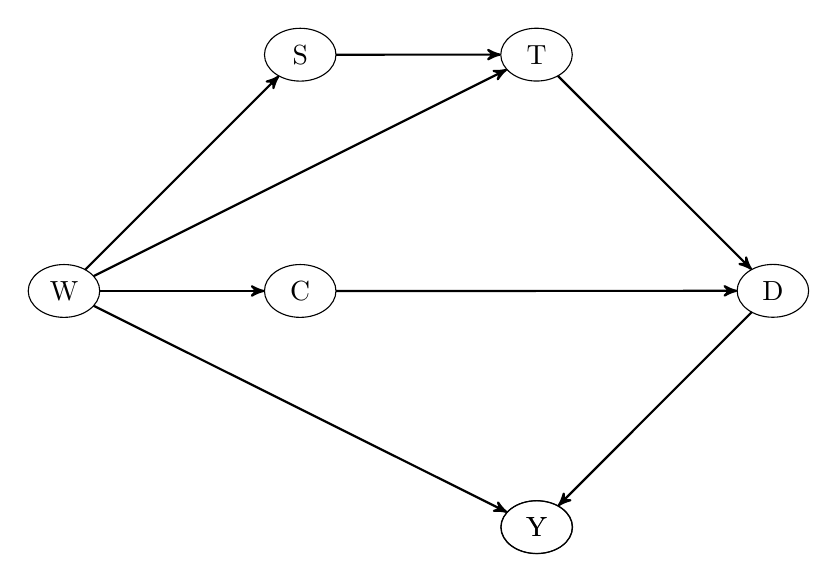
\begin{tikzpicture}[scale=1.5] 
\SetGraphUnit{2} 
\Vertex{W}  \NOEA(W){S} \EA(S){T}  \EA(W){C} \SOEA(T){D} \SOEA(C){Y} \SOWE(D){Y}
\Edges(W, S, T) \Edges(W,T) \Edges(W, C) \Edges(T, D) \Edges(C, D) \Edges(W, Y) \Edges(D, Y)
\end{tikzpicture}
\caption{Causal diagram indicating the conditional independence assumptions needed to estimate the PATT.}\label{fig:DAG}
\end{figure}

\begin{figure}[htbp]
\begin{center}
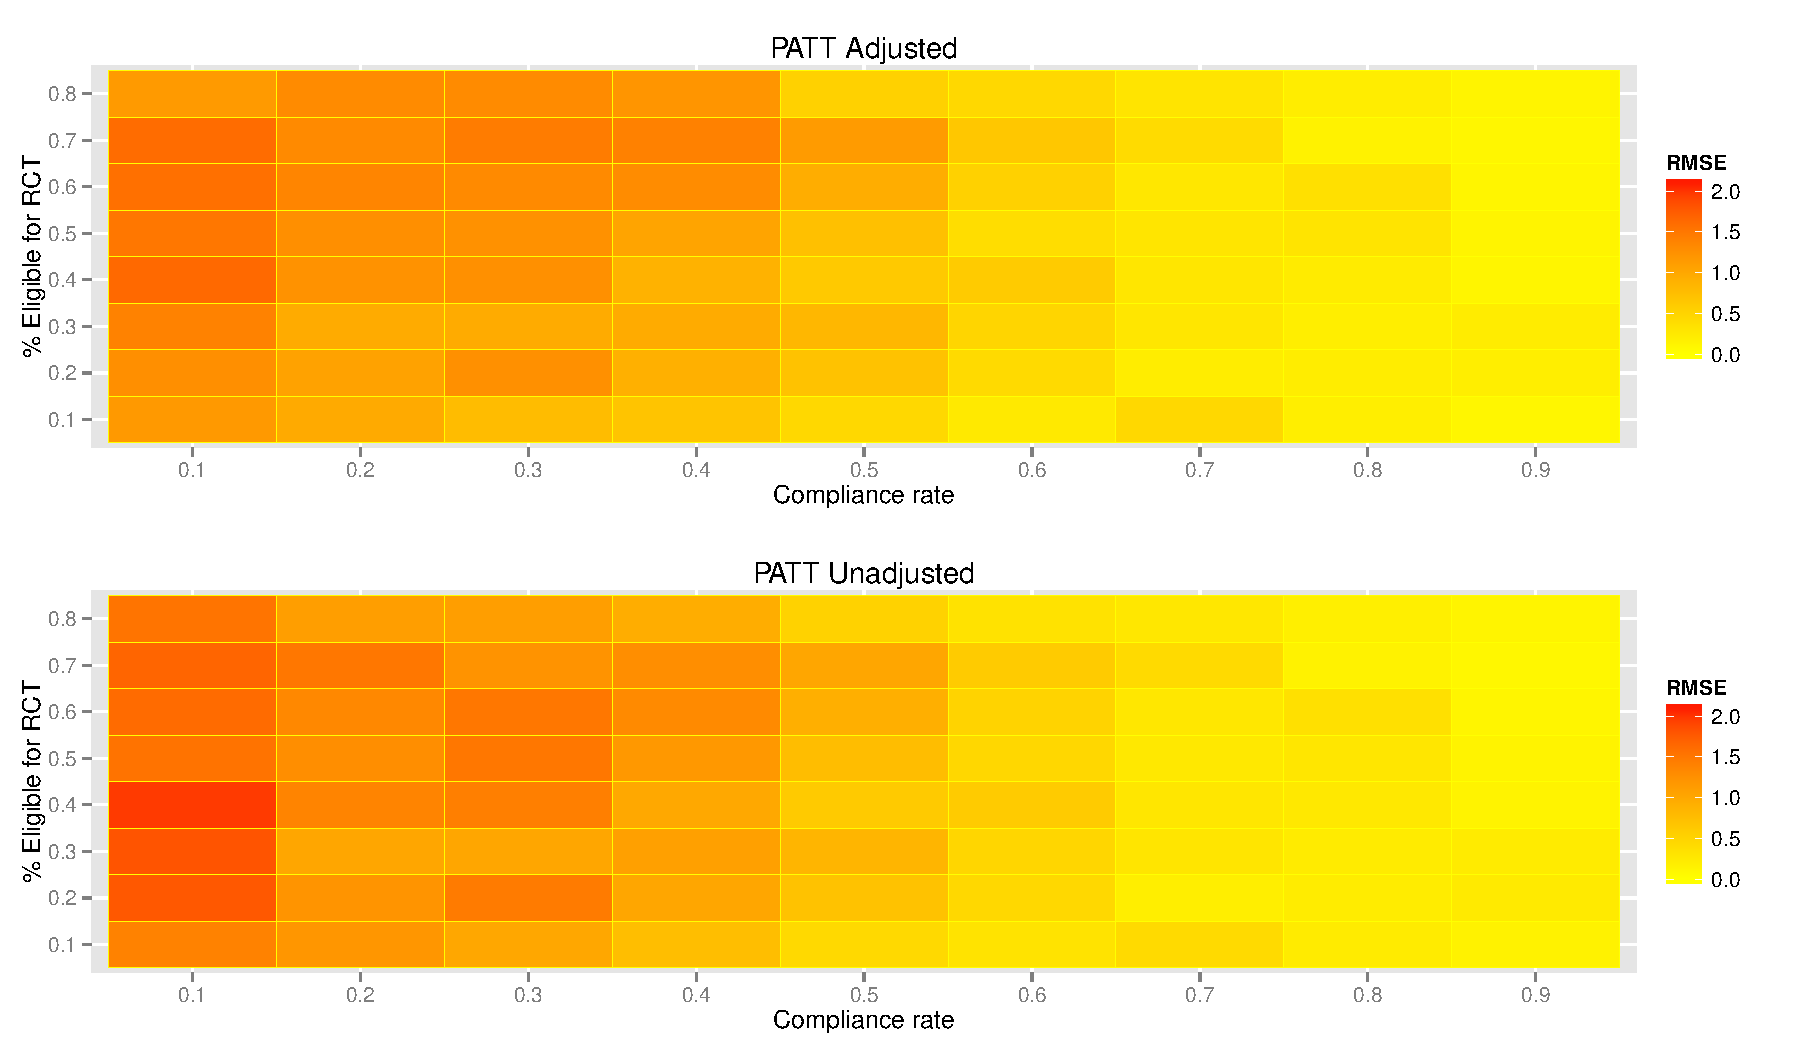
\includegraphics[width = 1\textwidth]{mse_ratec_rates_B5}
\caption{Simulation MSE, transformed by -$\log$. Darker tiles correspond to lower MSE.}
\label{fig:sim_tiles}
\end{center}
\end{figure}

\begin{figure}[htbp]
\begin{center}
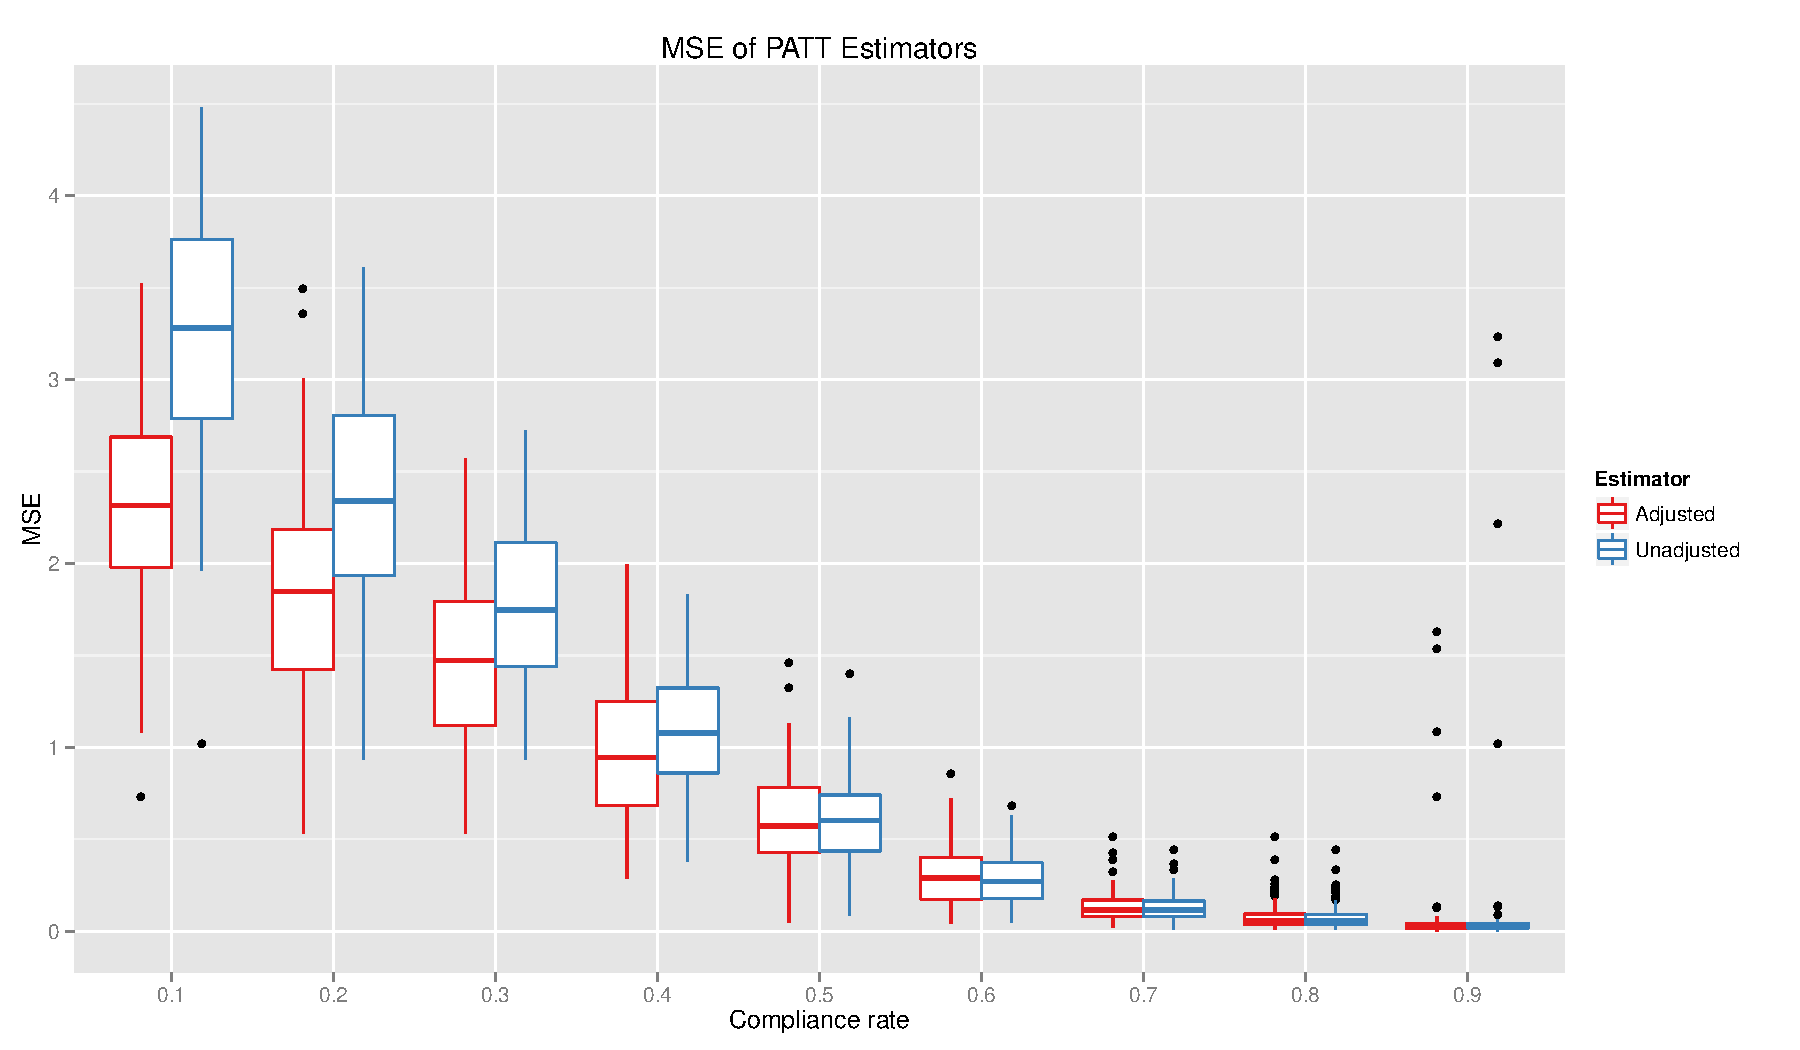
\includegraphics[width = 1\textwidth]{mse_boxplots_B5}
\caption{Simulation MSE, according to compliance rates in the total population.}
\label{fig:sim_compliance}
\end{center}
\end{figure}

\begin{singlespace}
\begin{longtable}{lllllll}
  & OHIE &  & OHIE &  & NHIS &  \\ 
    & control &  & treated &  &treated &   \\ 
  & $n=5476$ &  & $n=5193$ &  & $n=3382$ &  \\  
  \hline   
    \hline   
 \textbf{Covariate} &  $\mathbf{n}$ & $\mathbf{\%}$ & $\mathbf{n}$ & $\mathbf{\%}$ & $\mathbf{n}$ & $\mathbf{\%}$ \\ 
\hline
\textit{Sex:} &  & & &  &  & \\ 

\hspace{3mm} Female & 3148 & 57.5 & 2920 & 56.2 & 2380 & 70.4 \\ 
 &  & & &  &  & \\ 
\textit{Age:} &  & & &  &  & \\ 
\hspace{3mm}19-49 & 1636 & 29.9 & 1367 & 26.3 & 2429 & 71.8  \\ 

\hspace{3mm}50-64 & 3840 & 70.1 & 3826 & 73.7 & 953 & 28.2 \\ 
 &  & & &  &  & \\ 
\textit{Race:} &  & & &  &  & \\ 
\hspace{3mm}White & 4829 & 88.2 & 4393 & 84.6 & 1991 & 58.9  \\ 

\hspace{3mm}Black & 243 & 4.4 & 197 & 3.8 & 1050 & 31.1  \\ 

\hspace{3mm}Hispanic & 301 & 5.5 & 476 & 9.2 & 910 & 26.9  \\ 
 &  & & &  &  & \\ 
\textit{Health status:} &  & & &  &  & \\ 
\hspace{3mm}Diabetes & 581 & 10.6 & 539 & 10.4 & 452 & 13.4 \\ 

\hspace{3mm}Asthma & 1036 & 18.9 & 887 & 17.1 & 652 & 19.3  \\ 

\hspace{3mm}High blood pressure & 1670 & 30.5 & 1418 & 27.3 & 1143 & 33.8  \\ 
  
\hspace{3mm}Heart condition & 170 & 3.1 & 141 & 2.7 & 285 & 8.4 \\ 
 &  & & &  &  & \\ 
\textit{Education:} &  & & &  &  & \\  
\hspace{3mm}Less than high school  & 1056 & 19.3 & 950 & 18.3 & 1183 & 35.0  \\ 
  
\hspace{3mm}High school diploma or GED & 3081 & 56.3 & 2775 & 53.4 & 1076 & 31.8  \\ 

\hspace{3mm}Voc. training / 2-year degree & 969 & 17.7 & 1031 & 19.9 & 934 & 27.6 \\ 

\hspace{3mm}4-year college degree or more & 370 & 6.8 & 437 & 8.4 & 189 & 5.6 \\ 
 &  & & &  &  & \\ 
\textit{Income:} &  & & &  &  & \\ 
\hspace{3mm} $<\$10$k & 5476 & 100.0 & 3204 & 61.7 & 1452 & 42.9 \\

\hspace{3mm} \$10k-\$25k & 0 & 0.0 & 1616 & 31.1 & 1622 & 48.0 \\

\hspace{3mm} $>\$25$k & 0 & 0.0 & 373 & 7.2 & 308 & 9.1 \\
   \hline
\hline
 \textbf{Response} &   &  &  & &  &  \\ 
\hspace{3mm}Any ER visit &  1393 & 25.4 & 1301 & 25.1 & 881 & 26.1 \\ 
\hspace{3mm}Any outpatient visit & 3299 & 60.2 & 3081 & 59.3 & 2116 & 62.6 \\ 
\hline
\hline
\caption{Pretreatment covariates and responses for OHIE and NHIS respondents on Medicaid.} 
\label{rct-nrt-compare}
\end{longtable}
\end{singlespace}

\begin{figure}[htbp]
\begin{center}
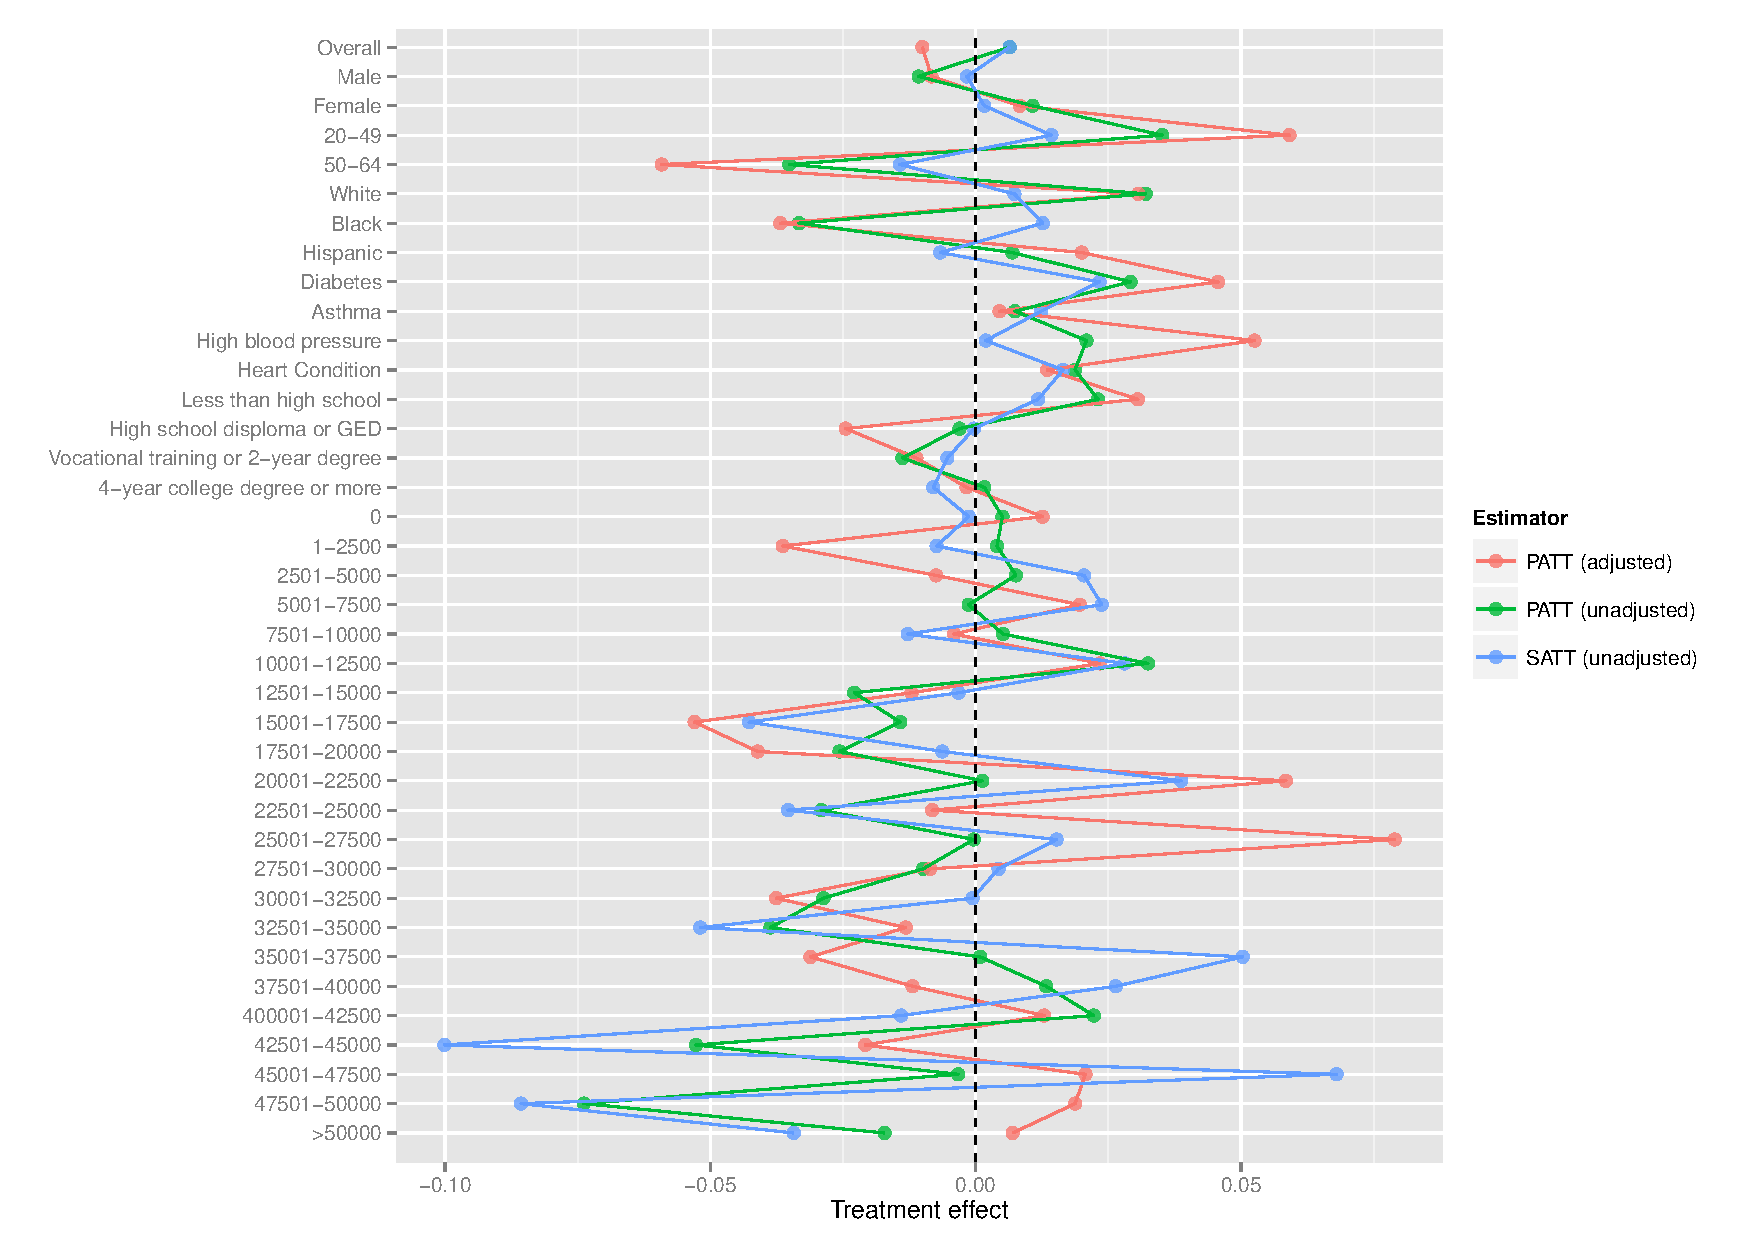
\includegraphics[width = 0.9\textwidth]{any-visit-plot.pdf}
    \caption{Comparison of estimators: any ER visit. Horizontal lines represent 95\% bootstrap confidence intervals.}
    \label{fig:any-visit-plot}
\end{center}
\end{figure}

\begin{figure}[htbp]
\begin{center}
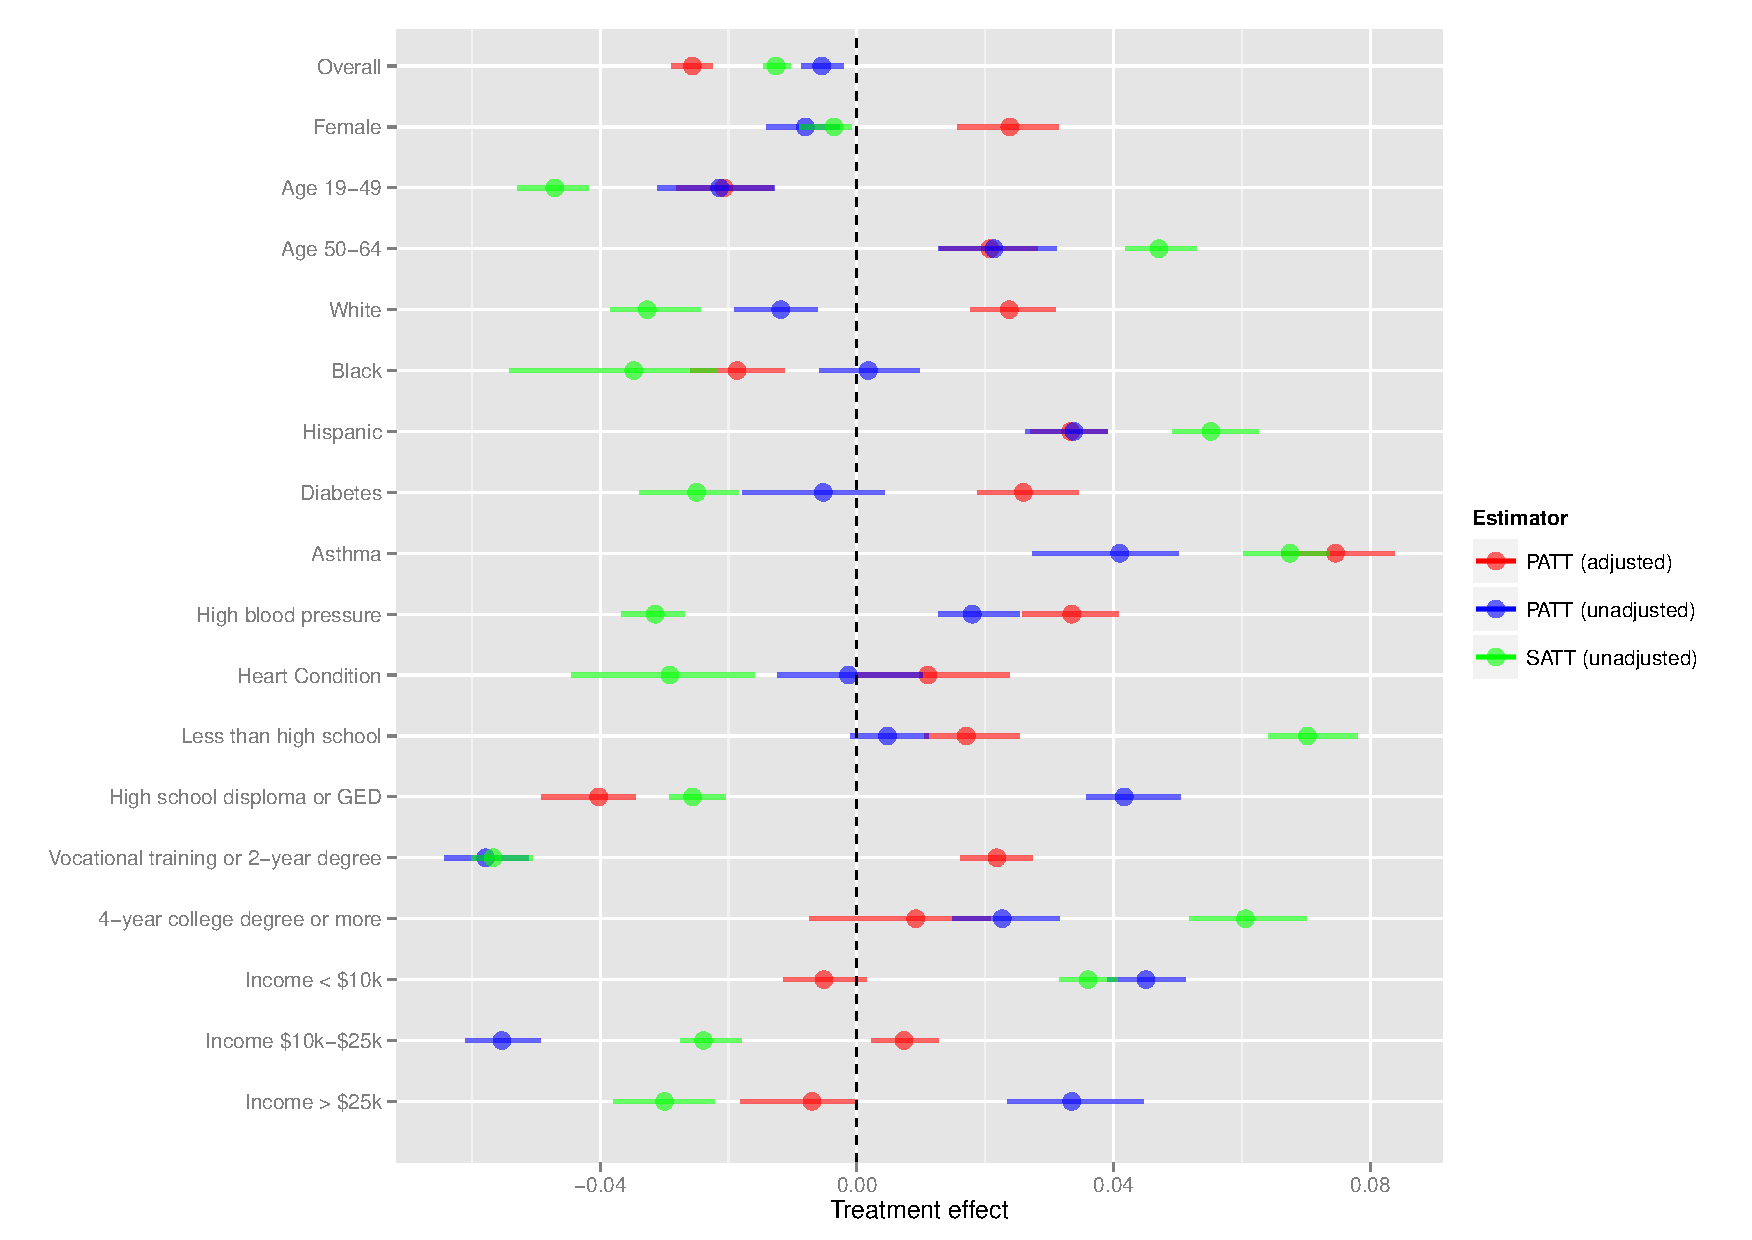
\includegraphics[width = 0.9\textwidth]{any-out-plot.pdf}
    \caption{Comparison of estimators: any outpatient visit. Horizontal lines represent 95\% bootstrap confidence intervals.}
    \label{fig:any-out-plot}
\end{center}
\end{figure}

\section{Ensemble method for compliance model}

% complier-mod
\begin{table}[htbp]
\begin{center}
\caption{Risk estimates for compliance model ensemble.} 
\label{compliance-ensemble}
\begin{tabular}{llcccc}
  \hline
 Algorithm & Parameters & Avg. & SE & Min. & Max. \\ 
  \hline
        \rowcolor{Gray}
Super Learner (\texttt{SuperLearner}) & default & 0.226 & 0.001 & 0.222 & 0.231 \\
%Discrete SL & default & 0.226 0.001 0.222 0.231 \\
Generalized boosted models (\texttt{gbm}) & default & 0.226 & 0.001 & 0.222 &  0.231 \\ 
Lasso regression (\texttt{glmnet})  & $\alpha=1$ & 0.227 & 0.001 & 0.224 & 0.233 \\ 
GLM with elasticnet regularization (\texttt{glmnet}) &  $\alpha=0.25$ & 0.227 & 0.001 & 0.224 & 0.232 \\ 
GLM with elasticnet regularization (\texttt{glmnet}) &  $\alpha=0.5$ & 0.227 & 0.001 & 0.224 & 0.233 \\ 
GLM with elasticnet regularization (\texttt{glmnet}) &  $\alpha=0.75$ & 0.227 & 0.001 & 0.224 & 0.233 \\ 
Neural network (\texttt{nnet}) &  default & 0.227 & 0.001 & 0.224 & 0.232 \\ 
Random forests (\texttt{randomForest}) & default & 0.307 & 0.003 & 0.293 & 0.326  \\  
Random forests (\texttt{randomForest})  & $\mathrm{mtry}=1$ & 0.273 & 0.002 & 0.268 & 0.281 \\ 
Random forests (\texttt{randomForest})  & $\mathrm{mtry}=5$  & 0.307 & 0.003 & 0.294 & 0.326 \\  
Random forests (\texttt{randomForest})  & $\mathrm{mtry}=10$ & 0.310 & 0.003 & 0.294 & 0.329 \\ 
Ridge regression (\texttt{glmnet}) &  $\alpha=0$ & 0.227 & 0.001 & 0.224 & 0.232 \\ 
   \hline
\end{tabular} 
\end{center}
\footnotesize{Note: risk based on the 10--fold cross-validated estimate of the MSE for each algorithm.}
\end{table}
%
%\pagebreak
%\section{Ensemble method for response models} 
%
%\subsection{Response model on RCT compliers}
%
%\begin{table}[htb]
%\caption{Cross--validated risk and weights used for each algorithm in super learner ensemble for response model on RCT compliers.}  \label{reponse-ensemble}
%  \begin{tabularx}{\linewidth}{l*{4}{Y}}
%    \toprule
%    \multicolumn{4}{l}{\textbf{Any ER visit}} \\
%    \midrule
% Algorithm & Parameters & Risk & Weight \\ 
%  \hline
%Generalized boosted models (\texttt{gbm}) & default & 0.188 & 0  \\ 
%Lasso regression (\texttt{glmnet})  & $\alpha=1$& 0.188 & 1 \\ 
%GLM with elasticnet regularization (\texttt{glmnet}) &  $\alpha=0.25$ & 0.188 & 0 \\ 
%GLM with elasticnet regularization (\texttt{glmnet}) &  $\alpha=0.5$ & 0.188 & 0 \\ 
%GLM with elasticnet regularization (\texttt{glmnet}) &  $\alpha=0.75$ & 0.188 & 0 \\ 
%Neural network (\texttt{nnet}) &  default & 0.234 & 0 \\ 
%        \rowcolor{Gray}
%Random forests (\texttt{randomForest}) & default & 0.24 & 0 \\ 
%Random forests (\texttt{randomForest})  & $\mathrm{mtry}=1$ & 0.251 & 0 \\ 
%Random forests (\texttt{randomForest})  & $\mathrm{mtry}=5$  & 0.24 & 0 \\ 
%Random forests (\texttt{randomForest})  & $\mathrm{mtry}=10$ & 0.241 & 0 \\ 
%Ridge regression (\texttt{glmnet}) &  $\alpha=0$ & 0.188 & 0 \\ 
%   \hline
%  \end{tabularx}
%  \begin{tabularx}{\linewidth}{l*{4}{Y}}
%    \toprule
%    \multicolumn{4}{l}{\textbf{Any outpatient visit}} \\
%    \midrule
%Generalized boosted models (\texttt{gbm}) & default & 0.24 & 0  \\ 
%Lasso regression (\texttt{glmnet})  & $\alpha=1$& 0.24 & 0 \\ 
%GLM with elasticnet regularization (\texttt{glmnet}) &  $\alpha=0.25$ & 0.24 & 0 \\ 
%GLM with elasticnet regularization (\texttt{glmnet}) &  $\alpha=0.5$ & 0.24 & 0.76 \\ 
%GLM with elasticnet regularization (\texttt{glmnet}) &  $\alpha=0.75$ & 0.24 & 0 \\ 
%Neural network (\texttt{nnet}) &  default & 0.242 & 0 \\ 
%        \rowcolor{Gray}
%Random forests (\texttt{randomForest}) & default & 0.331 & 0 \\ 
%Random forests (\texttt{randomForest})  & $\mathrm{mtry}=1$ & 0.392 & 0.23 \\ 
%Random forests (\texttt{randomForest})  & $\mathrm{mtry}=5$  & 0.333 & 0 \\ 
%Random forests (\texttt{randomForest})  & $\mathrm{mtry}=10$ & 0.333 & 0.008 \\ 
%Ridge regression (\texttt{glmnet}) &  $\alpha=0$ & 0.24 & 0 \\ 
%   \hline
%    \bottomrule
%  \end{tabularx}
%\footnotesize{`Risk' is the 10--fold cross-validated risk estimate based on MSE for each algorithm. `Weight' is the coefficient for the super learner, which is estimated using non--negative least squares based on the Lawson-Hanson algorithm.}
%\end{table}
%
%\pagebreak
%\subsection{Response model on all RCT participants}
%
%\begin{table}[htb]
%\caption{Cross--validated risk and weights used for each algorithm in super learner ensemble for response model on all RCT participants.}  \label{reponse-ensemble-unadj}
%  \begin{tabularx}{\linewidth}{l*{4}{Y}}
%    \toprule
%    \multicolumn{4}{l}{\textbf{Any ER visit}} \\
%    \midrule
% Algorithm & Parameters & Risk & Weight \\ 
%  \hline
%Generalized boosted models (\texttt{gbm}) & default & 0.188 & 0  \\ 
%Lasso regression (\texttt{glmnet})  & $\alpha=1$& 0.188 & 0.54 \\ 
%GLM with elasticnet regularization (\texttt{glmnet}) &  $\alpha=0.25$ & 0.188 & 0 \\ 
%GLM with elasticnet regularization (\texttt{glmnet}) &  $\alpha=0.5$ & 0.188 & 0 \\ 
%GLM with elasticnet regularization (\texttt{glmnet}) &  $\alpha=0.75$ & 0.188 & 0 \\ 
%Neural network (\texttt{nnet}) &  default & 0.228 & 0 \\ 
%   \rowcolor{Gray}
%Random forests (\texttt{randomForest}) & default & 0.24 & 0 \\ 
%Random forests (\texttt{randomForest})  & $\mathrm{mtry}=1$ & 0.252 & 0 \\ 
%Random forests (\texttt{randomForest})  & $\mathrm{mtry}=5$  & 0.241 & 0 \\ 
%Random forests (\texttt{randomForest})  & $\mathrm{mtry}=10$ & 0.241 & 0 \\ 
%Ridge regression (\texttt{glmnet}) &  $\alpha=0$ & 0.188 & 0.459 \\ 
%   \hline
%  \end{tabularx}
%  \begin{tabularx}{\linewidth}{l*{4}{Y}}
%    \toprule
%    \multicolumn{4}{l}{\textbf{Any outpatient visit}} \\
%    \midrule
%Generalized boosted models (\texttt{gbm}) & default & 0.239 & 0  \\ 
%Lasso regression (\texttt{glmnet})  & $\alpha=1$& 0.239 & 0 \\ 
%GLM with elasticnet regularization (\texttt{glmnet}) &  $\alpha=0.25$ & 0.239 & 0 \\ 
%GLM with elasticnet regularization (\texttt{glmnet}) &  $\alpha=0.5$ & 0.239 & 0 \\ 
%GLM with elasticnet regularization (\texttt{glmnet}) &  $\alpha=0.75$ & 0.239 & 0 \\ 
%Neural network (\texttt{nnet}) &  default & 0.24 & 0 \\ 
%   \rowcolor{Gray}
%Random forests (\texttt{randomForest}) & default & 0.327 & 0 \\ 
%Random forests (\texttt{randomForest})  & $\mathrm{mtry}=1$ & 0.391 & 0.261 \\ 
%Random forests (\texttt{randomForest})  & $\mathrm{mtry}=5$  & 0.331 & 0 \\ 
%Random forests (\texttt{randomForest})  & $\mathrm{mtry}=10$ & 0.329 & 0.008 \\ 
%Ridge regression (\texttt{glmnet}) &  $\alpha=0$ & 0.239 & 0.73 \\ 
%   \hline
%    \bottomrule
%  \end{tabularx}
%\end{table}

\end{appendices}

\itemize
\end{document}


